% Options for packages loaded elsewhere
\PassOptionsToPackage{unicode}{hyperref}
\PassOptionsToPackage{hyphens}{url}
%
\documentclass[
  man,mask]{apa7}
\usepackage{amsmath,amssymb}
\usepackage{lmodern}
\usepackage{iftex}
\ifPDFTeX
  \usepackage[T1]{fontenc}
  \usepackage[utf8]{inputenc}
  \usepackage{textcomp} % provide euro and other symbols
\else % if luatex or xetex
  \usepackage{unicode-math}
  \defaultfontfeatures{Scale=MatchLowercase}
  \defaultfontfeatures[\rmfamily]{Ligatures=TeX,Scale=1}
\fi
% Use upquote if available, for straight quotes in verbatim environments
\IfFileExists{upquote.sty}{\usepackage{upquote}}{}
\IfFileExists{microtype.sty}{% use microtype if available
  \usepackage[]{microtype}
  \UseMicrotypeSet[protrusion]{basicmath} % disable protrusion for tt fonts
}{}
\makeatletter
\@ifundefined{KOMAClassName}{% if non-KOMA class
  \IfFileExists{parskip.sty}{%
    \usepackage{parskip}
  }{% else
    \setlength{\parindent}{0pt}
    \setlength{\parskip}{6pt plus 2pt minus 1pt}}
}{% if KOMA class
  \KOMAoptions{parskip=half}}
\makeatother
\usepackage{xcolor}
\usepackage{graphicx}
\makeatletter
\def\maxwidth{\ifdim\Gin@nat@width>\linewidth\linewidth\else\Gin@nat@width\fi}
\def\maxheight{\ifdim\Gin@nat@height>\textheight\textheight\else\Gin@nat@height\fi}
\makeatother
% Scale images if necessary, so that they will not overflow the page
% margins by default, and it is still possible to overwrite the defaults
% using explicit options in \includegraphics[width, height, ...]{}
\setkeys{Gin}{width=\maxwidth,height=\maxheight,keepaspectratio}
% Set default figure placement to htbp
\makeatletter
\def\fps@figure{htbp}
\makeatother
\setlength{\emergencystretch}{3em} % prevent overfull lines
\providecommand{\tightlist}{%
  \setlength{\itemsep}{0pt}\setlength{\parskip}{0pt}}
\setcounter{secnumdepth}{-\maxdimen} % remove section numbering
% Make \paragraph and \subparagraph free-standing
\ifx\paragraph\undefined\else
  \let\oldparagraph\paragraph
  \renewcommand{\paragraph}[1]{\oldparagraph{#1}\mbox{}}
\fi
\ifx\subparagraph\undefined\else
  \let\oldsubparagraph\subparagraph
  \renewcommand{\subparagraph}[1]{\oldsubparagraph{#1}\mbox{}}
\fi
\newlength{\cslhangindent}
\setlength{\cslhangindent}{1.5em}
\newlength{\csllabelwidth}
\setlength{\csllabelwidth}{3em}
\newlength{\cslentryspacingunit} % times entry-spacing
\setlength{\cslentryspacingunit}{\parskip}
\newenvironment{CSLReferences}[2] % #1 hanging-ident, #2 entry spacing
 {% don't indent paragraphs
  \setlength{\parindent}{0pt}
  % turn on hanging indent if param 1 is 1
  \ifodd #1
  \let\oldpar\par
  \def\par{\hangindent=\cslhangindent\oldpar}
  \fi
  % set entry spacing
  \setlength{\parskip}{#2\cslentryspacingunit}
 }%
 {}
\usepackage{calc}
\newcommand{\CSLBlock}[1]{#1\hfill\break}
\newcommand{\CSLLeftMargin}[1]{\parbox[t]{\csllabelwidth}{#1}}
\newcommand{\CSLRightInline}[1]{\parbox[t]{\linewidth - \csllabelwidth}{#1}\break}
\newcommand{\CSLIndent}[1]{\hspace{\cslhangindent}#1}
\ifLuaTeX
\usepackage[bidi=basic]{babel}
\else
\usepackage[bidi=default]{babel}
\fi
\babelprovide[main,import]{english}
% get rid of language-specific shorthands (see #6817):
\let\LanguageShortHands\languageshorthands
\def\languageshorthands#1{}
% Manuscript styling
\usepackage{upgreek}
\captionsetup{font=singlespacing,justification=justified}

% Table formatting
\usepackage{longtable}
\usepackage{lscape}
% \usepackage[counterclockwise]{rotating}   % Landscape page setup for large tables
\usepackage{multirow}		% Table styling
\usepackage{tabularx}		% Control Column width
\usepackage[flushleft]{threeparttable}	% Allows for three part tables with a specified notes section
\usepackage{threeparttablex}            % Lets threeparttable work with longtable

% Create new environments so endfloat can handle them
% \newenvironment{ltable}
%   {\begin{landscape}\centering\begin{threeparttable}}
%   {\end{threeparttable}\end{landscape}}
\newenvironment{lltable}{\begin{landscape}\centering\begin{ThreePartTable}}{\end{ThreePartTable}\end{landscape}}

% Enables adjusting longtable caption width to table width
% Solution found at http://golatex.de/longtable-mit-caption-so-breit-wie-die-tabelle-t15767.html
\makeatletter
\newcommand\LastLTentrywidth{1em}
\newlength\longtablewidth
\setlength{\longtablewidth}{1in}
\newcommand{\getlongtablewidth}{\begingroup \ifcsname LT@\roman{LT@tables}\endcsname \global\longtablewidth=0pt \renewcommand{\LT@entry}[2]{\global\advance\longtablewidth by ##2\relax\gdef\LastLTentrywidth{##2}}\@nameuse{LT@\roman{LT@tables}} \fi \endgroup}

% \setlength{\parindent}{0.5in}
% \setlength{\parskip}{0pt plus 0pt minus 0pt}

% Overwrite redefinition of paragraph and subparagraph by the default LaTeX template
% See https://github.com/crsh/papaja/issues/292
\makeatletter
\renewcommand{\paragraph}{\@startsection{paragraph}{4}{\parindent}%
  {0\baselineskip \@plus 0.2ex \@minus 0.2ex}%
  {-1em}%
  {\normalfont\normalsize\bfseries\itshape\typesectitle}}

\renewcommand{\subparagraph}[1]{\@startsection{subparagraph}{5}{1em}%
  {0\baselineskip \@plus 0.2ex \@minus 0.2ex}%
  {-\z@\relax}%
  {\normalfont\normalsize\itshape\hspace{\parindent}{#1}\textit{\addperi}}{\relax}}
\makeatother

% \usepackage{etoolbox}
\makeatletter
\patchcmd{\HyOrg@maketitle}
  {\section{\normalfont\normalsize\abstractname}}
  {\section*{\normalfont\normalsize\abstractname}}
  {}{\typeout{Failed to patch abstract.}}
\patchcmd{\HyOrg@maketitle}
  {\section{\protect\normalfont{\@title}}}
  {\section*{\protect\normalfont{\@title}}}
  {}{\typeout{Failed to patch title.}}
\makeatother

\usepackage{xpatch}
\makeatletter
\xapptocmd\appendix
  {\xapptocmd\section
    {\addcontentsline{toc}{section}{\appendixname\ifoneappendix\else~\theappendix\fi\\: #1}}
    {}{\InnerPatchFailed}%
  }
{}{\PatchFailed}
\keywords{Survey methodology, sample weighting, nonresponse, response rate}
\DeclareDelayedFloatFlavor{ThreePartTable}{table}
\DeclareDelayedFloatFlavor{lltable}{table}
\DeclareDelayedFloatFlavor*{longtable}{table}
\makeatletter
\renewcommand{\efloat@iwrite}[1]{\immediate\expandafter\protected@write\csname efloat@post#1\endcsname{}}
\makeatother
\usepackage{lineno}

\linenumbers
\usepackage{csquotes}
\raggedbottom
\ifLuaTeX
  \usepackage{selnolig}  % disable illegal ligatures
\fi
\IfFileExists{bookmark.sty}{\usepackage{bookmark}}{\usepackage{hyperref}}
\IfFileExists{xurl.sty}{\usepackage{xurl}}{} % add URL line breaks if available
\urlstyle{same} % disable monospaced font for URLs
\hypersetup{
  pdftitle={Nonresponse and Sample Weighting in Organizational Surveying},
  pdflang={en-EN},
  pdfkeywords={Survey methodology, sample weighting, nonresponse, response rate},
  hidelinks,
  pdfcreator={LaTeX via pandoc}}

\title{Nonresponse and Sample Weighting in Organizational Surveying}
\author{John T. Kulas\textsuperscript{1}, Yang Yang\textsuperscript{2}, \& David H. Robinson\textsuperscript{3}}
\date{}


\shorttitle{NONRESPONSE AND SAMPLE WEIGHTING}

\authornote{

Correspondence concerning this article should be addressed to John T. Kulas, Dickson Hall \#250, Montclair State University, Montclair, NJ, 07043. E-mail: \href{mailto:kulasj@montclair.edu}{\nolinkurl{kulasj@montclair.edu}}

}

\affiliation{\vspace{0.5cm}\textsuperscript{1} Montclair State University\\\textsuperscript{2} Roche Group\\\textsuperscript{3} St.~Cloud State University}

\abstract{%
Post-stratification weighting is a common procedure used in public opinion polling applications to correct demographic constituency differences between samples and populations. Although common practice in public opinion polling, this form of data remediation is only sparsely acknowledged as a procedural topic worthy of empirical investigation within the organizational surveying literature. The current paper induces survey nonresponse via data simulation across fictional constituent groups (e.g., organizational strata) and documents the impact of weighting on the accuracy of sample statistics. Our goal was to evaluate the effectiveness of weighting when confronted with \emph{passive} and \emph{active} forms of nonresponse in an effort to: 1) interject this data-remediation procedure into the established organizational surveying literature focused on nonresponse, while also 2) exploring organizationally-relevant sampling scenarios that: a) benifit from, b) are ``hurt'' by, or c) are unaffected by post-stratification weighting. The results confirm that sampling contexts characterized by active nonresponse do benefit from application of sample weights, but only when accompanied by constituency differences in underlying population construct (e.g., surveyed \emph{attitude}) standing. Alternatively, constituent member differences in population attitudes, when characterized by passive forms of nonresponse, exhibit no benefit from weighting (in fact these scenarios are somewhat \emph{hurt} by weighting). The simulations reinforce that, moving forward, it would be prudent for surveyors of all disciplinary backgrounds to mutually attend to the traditional focus of both traditions: public opinion polling (e.g., multiple possible methodological sources of error as well as post-stratification adjustment) and organizational surveying (e.g., \emph{form} of nonresponse).
}



\begin{document}
\maketitle

Akin to differential variable weighting (for instance: a) construct indicators within an assessment scale {[}aka factor loadings{]}, or b) predictors within a selection system {[}aka regression weights{]}; e.g., per data matrix ``columns''), sample weighting alters the proportional contributions of \emph{individual respondents} within a data set (e.g., matrix rows). Some respondents' responses are assigned greater relative contribution and others are assigned less. This practice is commonplace in the summary of general population polling data reflecting, for example, elections and politics (e.g., Rivers \& Bailey, 2009), prevalence rates of psychological disorders (e.g., Kessler et al., 2009), or feelings of physical safety (e.g., Quine \& Morrell, 2008). It is also seemingly in the periphery of awareness and application within the published organizational surveying literature (see, for example, Kulas et al., 2016; Landers \& Behrend, 2015; Tett et al., 2014).

We speculate that this form of statistical remediation is gaining research interest in the organizational surveying research domain, at least in part, because industrial psychologists are keenly aware that response rates within organizational surveying applications have been trending downward (see, for example, Anseel et al., 2010; Rogelberg \& Stanton, 2007). With lower response rates, surveyors are confronted with heightened levels of scrutiny because, historically, a locally realized high response rate has been widely interpreted as a positive indicator of data quality - if not from the survey specialists themselves, at least from client stakeholders (e.g., Anseel et al., 2010; Cycyota \& Harrison, 2002, 2006; Frohlich, 2002).

The orientation of this presentation, however, is that although response rate is a commonly referenced proxy of survey quality, it is not response rate but rather sample \emph{representativeness} that should be the primary focus of concern for survey specialists (see, for example, Cook et al., 2000; Krosnick, 1999). Representativeness can of course be ``hurt'' by low response rates, but the relationship between these two survey concepts is by no means exact (e.g., Curtin et al., 2000; Keeter et al., 2006; Kulas et al., 2017). Stated differently, a high response rate is neither a sufficient nor even necessary condition for accurate population sampling.\footnote{There are indisputable benefits \emph{associated} with higher response rates, such as greater statistical \emph{power}. This benefit, however, should not be \emph{attributed to} response rate, but rather its consequence: larger \emph{n}. Our presentation reflects the fact that greater power (and/or, relatedly, smaller confidence intervals) may in fact introduce a \emph{false sense} of methodological superiority when the sample misrepresents the population. Primarily for this reason, we stress that the methodological/statistical concepts of response rate, sample size, and power need to be fully disentangled from the principle of representativeness, and the importance of these dissociations drives the central theme of the current paper.}

In the context of any survey application, sample/population misrepresentation ultimately refers to a discrepancy between estimated sample statistics and actual population parameters. Ideally, such discrepancies arise from completely random sources (in which case resulting error is less likely to be reasonably characterized as \emph{bias}). In reality, however, discrepancies are not only driven by purely random causes. There are several broader sampling methodology factors that may be systematically driving the relative under- or over-selection of a population segment (see, for example, Kulas et al., 2016), but the most commonly cited contributor within the organizational sciences is non-response (e.g., invited individuals simply either forget {[}e.g., passive nonresponse{]} or consciously choose not to participate in the survey process {[}e.g., active nonresponse{]}, see, for example, Rogelberg et al., 2000). Our presentation also focuses on this non-response contributor to sample misrepresentation, but only because we aim to: 1) integrate the organizational non-response and public-opinion post-stratification weighting literatures, while also 2) highlighting the associations and dissociations between response rate and bias (although we note here that the current presentation and procedure also inform other sampling methodological sources of misrepresentation than non-response).\footnote{Frequently presented as a separate consideration, \emph{measurement error} is an additional contributor to sample/population misrepresentation. The current focus is on deviations from a perfect sampling methodology as opposed to deviations from an ideal psychometric methodology. We do however note that future advancement of current representations of survey error would benefit from a unified perspective that encompasses error arising from both methodological sources: measurement and sampling strategy.}

\hypertarget{nonresponse-in-organizational-surveying}{%
\subsection{Nonresponse in Organizational Surveying}\label{nonresponse-in-organizational-surveying}}

Within the organizational surveying domain, it is not uncommon for response rate (RR) to be referenced as a proxy for survey data quality (see, for example, Baruch \& Holtom, 2008; Fan \& Yan, 2010; Pedersen \& Nielsen, 2016). Baruch (1999), for example, states that, ``\ldots to have dependable, valid, and reliable results, we need a high RR from a wide representation of the whole population under study'' and that, ``The level of RR is an important, sometimes crucial, issue in relation to the validity of a paper's results'' (p.~422). Fan and Yan (2010) similarly state that response rate is, ``\ldots the most widely used and commonly computed statistic to indicate the quality of surveys'' (p.~132). Pedersen and Nielsen (2016) claim that a high survey response rate, ``\ldots diminishes sampling bias concerns and promotes the validity of survey-based research findings'' (p.~230). The general consensus seems to be that there are three major (negative) consequences of low response rates, including (a) yielding smaller sample size, which negatively impacts statistical power and confidence intervals, (b) reducing the credibility of survey data, and (c) generating biased samples that impair the generalizability of survey results (Biemer \& Lyberg, 2003; Luong \& Rogelberg, 1998; Rogelberg et al., 2000).

To the likely frustration of those who associate response rate with survey data quality, organizational survey response rates have, on average, been declining for decades. Baruch (1999), for example, summarized response rates of 175 studies published in five leading management and behavioral sciences journals in 1975, 1985, and 1995. His results revealed an average response rate (across time periods) of 55.6\% (\emph{SD} = 19.7\%), but also a trend within which response rates declined steadily from 64.4\% to 55.7\% to 48.4\% over the three time points. Nine years later, Baruch and Holtom (2008) conducted a follow-up study of 1,607 studies published in 17 disciplinary-relevant journals in 2000 and 2005 but found no substantial differences in response rates compared to those in 1995, suggesting that the declining trend had perhaps reached a lower asymptote. However, a different approach with similar goals (Anseel et al., 2010) analyzed 2,037 survey projects published in 12 journals in Industrial and Organizational Psychology, Management, and Marketing from 1995 to 2008 and did note a slight decline (overall \emph{M} = 52.3\%) when controlling for the use of response enhancing techniques.\footnote{It is possible that the declination has stabilized with mean response rates hovering around 50\% after roughly the turn of the millenium (\emph{M} = 52.5\% for HRM studies from 2009 to 2013, Mellahi \& Harris, 2016; \emph{M} = 52.0\% for management studies from 2000 to 2004, Werner et al., 2007). This stability, if authentic, may again possibly be accounted for by an increased contemporary emphasis on response enhancing strategies (Anseel et al., 2010; Fulton, 2016).}

\hypertarget{form-of-nonresponse}{%
\subsubsection{\texorpdfstring{\emph{Form} of Nonresponse}{Form of Nonresponse}}\label{form-of-nonresponse}}

Although high response rates are generally pursued as a desirable goal within organizational surveying applications, there has also been a broad acknowledgement that not all forms of nonresponse should be considered equally worrisome. Rogelberg et al. (2003), for example, propose a distinction between \emph{active} and \emph{passive} nonrespondents based on intent and (in)action. According to Rogelberg et al. (2003), active nonrespondents are those who intentionally refuse to participate in surveys, while passive nonrespondents are those who fail to respond to surveys due to reasons such as forgetting or misplacing invitations. Passive nonrespondents are thought to be similar to respondents in both attitude (Rogelberg et al., 2003) as well as organizational citizenship behaviors (OCBs, Spitzmüller et al., 2007), whereas active nonrespondents have been shown to exhibit significantly lower organizational commitment and satisfaction, higher intention to quit, lower conscientiousness, and lower OCBs than actual respondents (Rogelberg et al., 2000, 2003; Spitzmüller et al., 2007).

The more commonly encountered form of organizational nonresponse appears to be passive (Rogelberg et al., 2003; Rogelberg \& Stanton, 2007), although subgroup rates may evidence variability - men, for example, have a higher proclivity toward active nonresponse than do women (Luong \& Rogelberg, 1998; Rogelberg et al., 2000; Spitzmüller et al., 2007). Additionally, it has been noted that selection of an individual population element into a realized sample is often predictable (because of, for example, an increased likelihood of not responding when dissatisfied or disgruntled, Taris \& Schreurs, 2007). The organizational surveying expectation is that, \emph{on average}, roughly 15\% of nonrespondents should be expected to be accurately characterized as ``active'' (Rogelberg et al., 2003; Rogelberg \& Stanton, 2007; Werner et al., 2007). It is this second, less frequently anticipated form of nonresponse that also carries the greater corresponding threat of biased sample estimates (see, for example, Kulas et al., 2017; Rogelberg \& Stanton, 2007).

\hypertarget{sample-weighting---a-brief-overview}{%
\section{Sample Weighting - a Brief Overview}\label{sample-weighting---a-brief-overview}}

Within public opinion polling contexts, when realized sample constituencies (e.g., 44\% male - by tradition from \emph{judisciously-constructed} and \emph{randomly sampled} data frames)\footnote{These important sampling concepts are very carefully attended to within public opinion polling contexts. Conversely, within organizational surveying traditions, these considerations are not commonly acknowledged, at least explicitly within the published literature. The weighting procedure presented in the current manuscript remediates bias regardless of full methodological consideration of sampling context, but is dependent on accurate ``census'' population constituency estimates (and, as the results highlight, the presence of an active nonrespondent group). Although beyond the scope of the current project, an acknowledgement of the broader methodological sampling context, and the additional potential sources of error, facilitates a deeper appreciation and understanding of the benefits and potential pitfalls of sample weighting.} are compared against census estimates of population parameters (e.g., 49\% male), weights are applied to the realized sample in an effort to remediate the relative proportional under- or over-sampling. This is because, if the broader populations from which the under- or over-represented groups are sampled differ along surveyed dimensions (e.g., males, within the population, are \emph{less likely to vote for Candidate X} than are women), then unweighted aggregate statistics (of, for example, projected voting results) will misrepresent the true population parameter. This remedial application of sample weights should also be considered an option for organizational researchers pursuing answers to similar survey questions such as: ``What is the mood of the employees?'' This is because focused queries such as this are (perhaps somewhat covertly) layered - implicit in the question is a focus not on survey results, but rather the broader employee population. Acknowledging this implicit target group is of course important, because the next step (after gauging the mood of the surveyed respondents) is \emph{doing something} about it. Weighting should be considered a procedural option for organizational surveyors to potentially transition a bit closer from, ``What do the survey results say''? to ``What do the employees feel''?

\hypertarget{procedural-application}{%
\subsection{Procedural application}\label{procedural-application}}

\emph{Proportional weights} are the form of weights most directly relevant to organizational surveying applications that traditionally focus on nonresponse as the primary contributor to sample misrepresentation. These weights are ratios of the proportion of a population within a given stratum to the proportion of the sample within that same stratum:

\begin{equation}
proportional \: weight(\pi_k) = \frac{(N_k/N)}{(n_k/n)}
\end{equation}

Over-sampling of elements of a stratum (\emph{k}) results in proportional weights less than one, while under-sampling (relative to the population) results in proportional weights greater than one.
The common procedure for weight estimation \emph{when more than one stratum is specified} is an iterative process that may be referred to by multiple substantively synonymous terms: \emph{rim weighting}, \emph{iterative proportional fitting}, or \emph{raking} (see, for example, Deming \& Stephan, 1940). Regardless of label, the procedure guides the surveyor to:

\begin{enumerate}
\def\labelenumi{\arabic{enumi})}
\item
  Determine proportional weights for all levels within one stratum, and then assign these weights to cases.
\item
  Determine proportional weights for a second group (ratio of population percent to \emph{current} sample percent {[}the current sample percent will be affected by the step 1 weighting procedure{]}). Multiply previous (step 1) weights by the proportional weights for this second stratum and assign these new weights to cases.
\item
  Determine proportional weights for a third stratum (which will once again require re-inspection of the \emph{current} sample percent). Multiply the previous step 2 weights by the third stratum proportional weights and assign to cases.
\item
  Iterate through steps 1, 2, and 3 (or more if more than three strata are considered) until the weighted sample characteristics match the population characteristics.
\end{enumerate}

Possible strata relevant for organizational survey weighting include: branch, full-, part-, or flex-time status, functional area, gender, geographic location, hierarchy, remote-working categorization, salaried status, subsidiary, tenure, work shift, or any other groupings especially deemed suspect to possess a relatively disporportionate number of active nonrespondents (through application of forecasting strategies such as those advocated by, for example, Rogelberg and Stanton, 2007). Each of these strata may of course also be the targeted focus of survey results feedback, but when \emph{aggregating} results across (or even within) strata, a consideration of the impact of nonresponse \emph{has the potential} to yield more accurate survey estimates. The explicit goal is therefore a closer approximation of sample descriptives to population parameters via statistical remediation, and drives the current paper's focus on the interplay of four survey concepts (distribution of attitude within the larger population, response rate, nonresponse form, and remedial weighting).

\emph{Research question 1}: What role does overall response \emph{rate} play in sample/population misrepresentation? \textbf{{[}make sure this is reflected in results{]}}

\emph{Research question 2}: What role does nonresponse \emph{form} (passive versus active) play in sample/population misrepresentation? \textbf{currently in paper as figures 1-3}

\emph{Research question 3}: What impact does the application of weights have on both biased (e.g., misrepresentative) and unbiased sample estimates?

\emph{Research question 4}: What is the role of response rate, form, and underlying population attitudes in the \emph{effectiveness} of weighting? \textbf{{[}perhaps David can derive/find a proof to parallel our results?{]}}

\begin{quote}
Added population attitudes (1/20/23) - not sure if this clutters but more consistent with flow of introduction
\end{quote}

We view these questions as being analogous to similar questions asked and answered with differential variable weighting within the broader applied psychological disciplines. Just as, for example, there has been debate regarding the merits of differential versus unit variable weighting in a selection context (e.g., Wainer, 1976) or simple composite score aggregate (Bobko et al., 2007), we propose that a similar consideration is appropriate with persons, and therefore compare and contrast unit- versus variable-sample element weighting via carefully controlled data simulation.

\hypertarget{methods}{%
\section{Methods}\label{methods}}

We address our research questions within the context of organizational surveying (commonly assessing estimates of, for example, commitment, culture/climate, engagement, or satisfaction). We began the simulations by establishing ``populations'', each consisting of 10,000 respondents characterized by demographic categorizations across gender (male and female) and department (A and B). We therefore had four demographic groups (male-A, male-B, female-A, and female-B). For these population respondents, we generated scaled continuous responses (real numbers) ranging from values of 1 to 5, reflecting averaged aggregate scale scores from a fictional multi-item survey with a typical 1 \(\rightarrow\) 5 Likert-type or graphic rating scale response format.

In order to represent different proportions of relative constituency (for example, more females than males or more department A workers than department B), we iterated population characteristics at marginal levels (gender and department) starting at 20\% (and 80\%) with increments and corresponding decriments of 20\%. For example, if males accounted for 20\% of the simulated population, then females were 80\%; also if respondents in Department A represented 60\% of a population, then 40\% were in Department B. Marginal constituencies were therefore specified at all combinations (across the two variables) of 20\% and 80\%, 40\% and 60\%, 60\% and 40\%, and 80\% and 20\%. This resulted in population \emph{cell} constituencies (e.g., men in department A) as low as 400 and as high as 6,400.

\begin{table}[tbp]

\begin{center}
\begin{threeparttable}

\caption{\label{tab:Tab1}Attitudinal Distribution Conditions Specified in Current Paper}

\small{

\begin{tabular}{clcccccc}
\toprule
 &  &  & \multicolumn{2}{c}{Male} & \multicolumn{2}{c}{Female}  &\\
\cmidrule(r){4-5} \cmidrule(r){6-7}
Condition & Distributional Shape & mu & Dept A & Dept B & Dept A & Dept B & Anticipated Bias\\
\midrule
1 & Normal & 3 & X & X & X & X & None\\
 & Positive Skew & 2 &  &  &  &  & \\
 & Negative Skew & 4 &  &  &  &  & \\
2 & Normal & 3 &  &  &  &  & None\\
 & Positive Skew & 2 & X & X & X & X & \\
 & Negative Skew & 4 &  &  &  &  & \\
3 & Normal & 3 &  &  &  &  & None\\
 & Positive Skew & 2 &  &  &  &  & \\
 & Negative Skew & 4 & X & X & X & X & \\
4 & Normal & 3 & X & X & X &  & Moderate\\
 & Positive Skew & 2 &  &  &  &  & \\
 & Negative Skew & 4 &  &  &  & X & \\
5 & Normal & 3 & X & X &  &  & Moderate/High\\
 & Positive Skew & 2 &  &  & X & X & \\
 & Negative Skew & 4 &  &  &  &  & \\
6 & Normal & 3 &  & X & X &  & Moderate/High\\
 & Positive Skew & 2 & X &  &  &  & \\
 & Negative Skew & 4 &  &  &  & X & \\
7 & Normal & 3 &  &  &  &  & High\\
 & Positive Skew & 2 & X &  & X &  & \\
 & Negative Skew & 4 &  & X &  & X & \\
8 & Normal & 3 &  &  &  &  & High\\
 & Positive Skew & 2 & X & X &  &  & \\
 & Negative Skew & 4 &  &  & X & X & \\
\bottomrule
\end{tabular}

}

\end{threeparttable}
\end{center}

\end{table}

Additionally, each of these cell populations was characterized by an attitude distribution in one of three different possible forms: normal, positively skewed, or negatively skewed. These distributional forms were specified in an attempt to model similarities and discrepancies in construct standing (e.g., commitment, satisfaction, or engagement) across respondent groupings. The normal distribution exhibited, on average, a mean of 3.0 whereas the skewed distributions were characterized by average means of 2.0 and 4.0, respectively. In total, eight crossings of distributional type across employee categorization were specified (Table \ref{tab:Tab1} presents the combinations of these distributions). Note that these eight conditions are not exhaustive of all possible combinations - we specified scenarios that we expected to be most efficiently informative across our passive to active nonresponse continuum (reflected in Table \ref{tab:Tab1}'s ``anticipated bias'' column).

Individual attitudes were randomly sampled from population distributions at the cell level (e.g., Department A Males) without replacement. Response rates (methodologially these could also be conceptualized as \emph{sampling} rates) were controlled at the marginal level using 10\% increments ranging from 60\% to 90\%, and these were fully iterated. Our cell-level response rates therefore ranged from 36\% to 81\% - a range of rates chosen because they are, according to the organizational surveying literature, reasonable expectations (e.g., Mellahi \& Harris, 2016; Werner et al., 2007). We therefore investigated error within the aggregate mean (e.g., grand mean or total sample mean) attributable to different likelihoods of sample inclusion from constituent groups of different relative size and representing populations of different attitudinal distribution, but at response rates reasonably expected to exist in real-world organizational surveying contexts.

It should be noted here that there are several collective patterns of response that are intended to represent sampling scenarios exhibiting \emph{passive} nonresponse, regardless of absolute response rate: all subgroups exhibiting the same response rate (e.g., 36\%, 36\%, 36\%, and 36\%). All other combinations of response rate are intended operationalizations of active forms of nonresponse (e.g., \emph{not} reasonably characterized as missing at random, NMAR), although the degree to which a sampling scenario should be reasonably characterized as exhibiting active nonresponse is intended to be incremental across iterations.

\begin{lltable}

\small{

\begin{longtable}{ccccccc}\noalign{\getlongtablewidth\global\LTcapwidth=\longtablewidth}
\caption{\label{tab:Tab2}Example Summarized Response Rate Conditions Represented in Figures 2 through 5}\\
\toprule
 \multicolumn{4}{c}{Example Response Rates (Any Combination)}  &  &  &\\
\cmidrule(r){1-4}
Male Dept A & Male Dept B & Female Dept A & Female Dept B & SD Index & Number of Conditions & Form (and degree) of Nonresponse\\
\midrule
\endfirsthead
\caption*{\normalfont{Table \ref{tab:Tab2} continued}}\\
\toprule
 \multicolumn{4}{c}{Example Response Rates (Any Combination)}  &  &  &\\
\cmidrule(r){1-4}
Male Dept A & Male Dept B & Female Dept A & Female Dept B & SD Index & Number of Conditions & Form (and degree) of Nonresponse\\
\midrule
\endhead
36\% & 36\% & 36\% & 36\% & .000 & 256 & Passive\\
36\% & 36\% & 42\% & 42\% & .034 & 128 & \\
48\% & 48\% & 54\% & 54\% & .035 & 64 & \\
42\% & 42\% & 49\% & 49\% & .040 & 192 & \\
48\% & 48\% & 56\% & 56\% & .046 & 128 & \\
56\% & 56\% & 64\% & 64\% & .047 & 64 & \\
54\% & 54\% & 63\% & 63\% & .051 & 128 & \\
63\% & 63\% & 72\% & 72\% & .052 & 64 & \\
36\% & 42\% & 42\% & 49\% & .053 & 64 & \\
42\% & 48\% & 49\% & 56\% & .057 & 128 & \\
49\% & 56\% & 56\% & 64\% & .061 & 64 & \\
48\% & 54\% & 56\% & 63\% & .062 & 128 & \\
56\% & 63\% & 64\% & 72\% & .066 & 128 & \\
36\% & 36\% & 48\% & 48\% & .069 & 128 & \\
64\% & 72\% & 72\% & 81\% & .069 & 64 & \\
42\% & 42\% & 56\% & 56\% & .081 & 128 & \\
36\% & 42\% & 48\% & 56\% & .085 & 128 & \\
42\% & 49\% & 54\% & 63\% & .089 & 128 & \\
48\% & 48\% & 64\% & 64\% & .092 & 128 & \\
42\% & 48\% & 56\% & 64\% & .096 & 128 & \\
49\% & 56\% & 63\% & 72\% & .098 & 128 & \\
36\% & 36\% & 54\% & 54\% & .104 & 192 & \\
48\% & 54\% & 64\% & 72\% & .106 & 128 & \\
56\% & 63\% & 72\% & 81\% & .109 & 128 & \\
36\% & 48\% & 48\% & 64\% & .115 & 64 & \\
36\% & 42\% & 54\% & 63\% & .120 & 128 & \\
42\% & 42\% & 63\% & 63\% & .121 & 64 & \\
42\% & 54\% & 56\% & 72\% & .123 & 128 & \\
49\% & 63\% & 63\% & 81\% & .131 & 64 & \\
42\% & 48\% & 63\% & 72\% & .137 & 128 & \\
48\% & 48\% & 72\% & 72\% & .139 & 64 & \\
36\% & 48\% & 54\% & 72\% & .150 & 128 & \\
48\% & 54\% & 72\% & 81\% & .154 & 128 & \\
54\% & 54\% & 81\% & 81\% & .156 & 64 & \\
42\% & 54\% & 63\% & 81\% & .164 & 128 & \\
36\% & 54\% & 54\% & 81\% & .186 & 64 & Active\\
\bottomrule
\end{longtable}

}

\end{lltable}

In an attempt to capture this ``degree of active nonresponse'', we calculated a simple index of response rate discrepancy (SD; presented in Table \ref{tab:Tab2}). The ``least'' active nonresponse scenarios are characterized by two subgroups with identical response rates and two having a slightly different response rate (e.g., Dept A Males = 36\%, Dept A Females = 36\%, Dept B Males = 42\%, and Dept B Females = 42\%; see the second row of Table \ref{tab:Tab2}, the SD index = .034)\footnote{This method of simplifying the presentation of our response rate conditions is fully orthogonal to population constituency and distributional form. That is, the amount of bias present in a sample estimate is expected to be quite different for Condition 7 with response rates of 48\%, 48\%, 72\%, 72\% versus 48\%, 72\%, 48\%, 72\%, even though the crude response rate index (SD = 0.139) is the same for both scenarios. There is additional information within these simulations (the effect of a \emph{combination} of response rate and population form on degree of bias) that is therefore not captured via this simple SD index.}. Also here note that three of our eight Table \ref{tab:Tab1} conditions represent scenarios where the presence of active nonrespondents is not expected to result in bias (e.g., regardless of patterns of nonresponse, the unweighted sample mean is expected to yield an unbiased estimate of the population mean). These are Table \ref{tab:Tab1} conditions one through three, where attitudinal distributions are of \emph{the same form} across groups, regardless of any individual group response rate discrepancy from others'.

These operationalizations of passive and active forms of nonresponse differ from other investigations with similar goals. Kulas et al. (2017), for example, directly tie probabilities of sample inclusion to an individual's held attitude (the likelihood of sample inclusion is fully dependent on the population member's attitude). Conversely, the probability of sample inclusion in the current investigation is dependent only on \emph{group} membership (with some of these groups occasionally being characterized by unique attitude distributional forms). Essentially, Kulas et al. (2017) operationalize active nonresponse at the person-level whereas the current paper does so at the group level. This may be a more appropriate procedural specification with regard to the implications of these simulations, as organizational surveyors are more likely to have an inclination of a group's collective attitude or likelihood to respond (e.g., night shift workers, machine operators) than they are of any one individual employee.

\hypertarget{results}{%
\section{Results}\label{results}}

In total, we generated 327.68 million samples (4,096 unique combinations of response rate and population constituency across gender and department, simulated 10,000 times each across our eight Table \ref{tab:Tab1} conditions). Each of these samples was comprised of, on average, \emph{n} = 5,625, collectively representing an experiment-wide simulated \emph{n} of 1.8432 trillion. For each individual simulation, weights were applied iteratively to the data at the two marginal (variable) levels via raking, and were estimated via the \emph{anesrake} package (Pasek, 2018) in R version 4.2.2 (2022-10-31 ucrt).

We were most interested in comparing the extent to which unweighted (aggregated responses without raking) and weighted (aggregated weighted responses) sample means approximated the population means across our controlled specifications of response rate, nonresponse form, and attitudinal distribution. Population means were taken from each iteration, as the simulations specified a new population at each iteration. The ``misrepresentation'' betwen sample and population was operationalized by calculating: 1) the discrepancies between the population and both weighted and unweighted sample means, as well as, 2) the averaged deviations of these discrepancies from the population mean (discrepancy in the ``mean'' of the means is bias, dispersion about the ``mean'' of the means is error). If the average weighted sample mean was closer to the true population mean, relative to the unweighted one, then the weighting was deemed beneficial.

\hypertarget{role-of-overall-response-rate}{%
\subsection{Role of overall response rate}\label{role-of-overall-response-rate}}

Research question \#1 asked what role overall response rate plays in sample/population misrepresentation.

Correlation coefficient needed.{[}Yang to calculate 2/1{]}
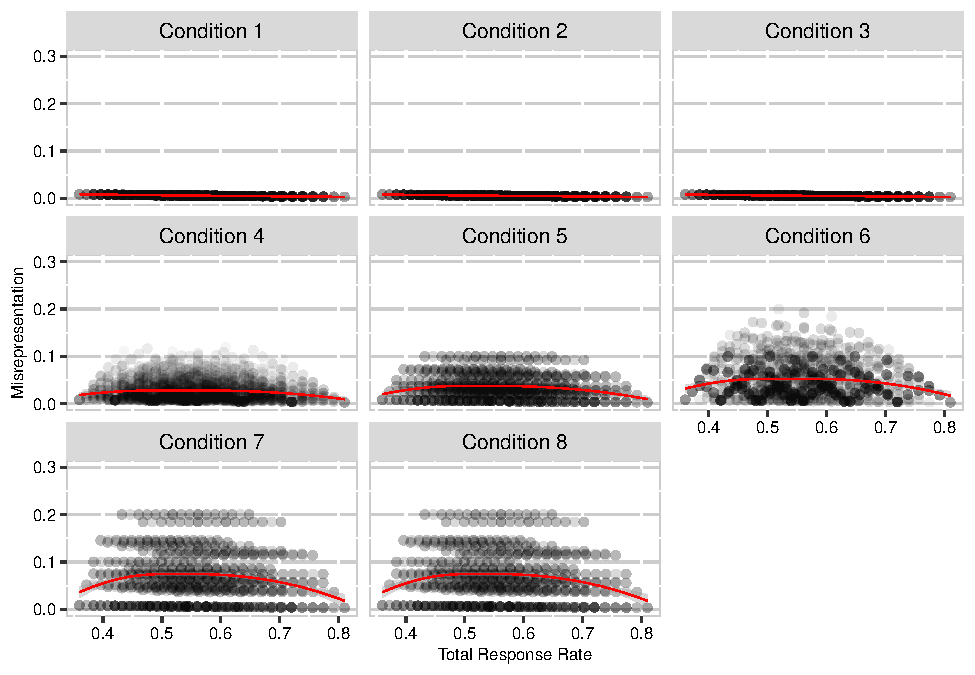
\includegraphics{Simulation-paper2-20200207_files/figure-latex/Figure1-1.pdf}

\begin{figure}
\centering
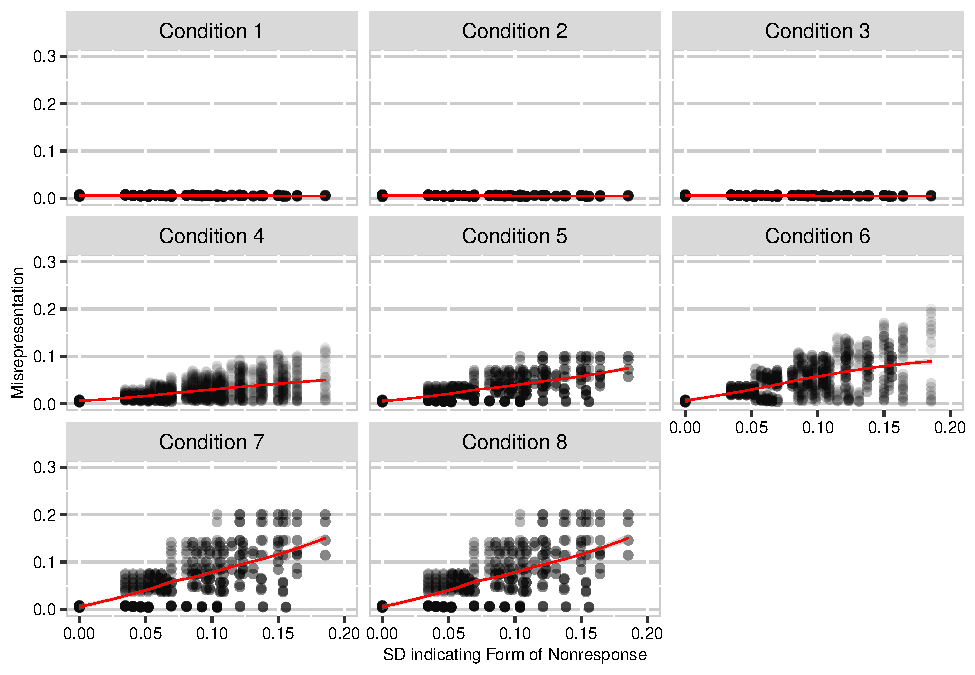
\includegraphics{Simulation-paper2-20200207_files/figure-latex/Figure2-1.pdf}
\caption{\label{fig:Figure2}Relationship between nonresponse form and misrepresentation.}
\end{figure}

\begin{figure}
\centering
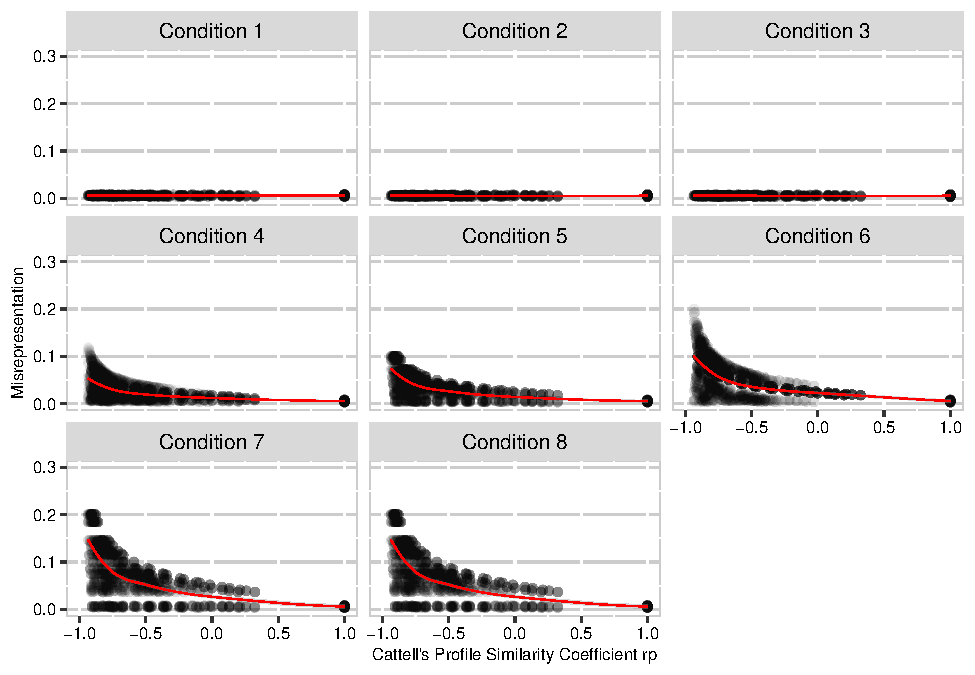
\includegraphics{Simulation-paper2-20200207_files/figure-latex/Figure3-1.pdf}
\caption{\label{fig:Figure3}Relationship between sample representativeness and misrepresentation.}
\end{figure}

\begin{verbatim}
## Warning: The `size` argument of `element_rect()` is deprecated as of ggplot2 3.4.0.
## i Please use the `linewidth` argument instead.
\end{verbatim}

\begin{figure}
\centering
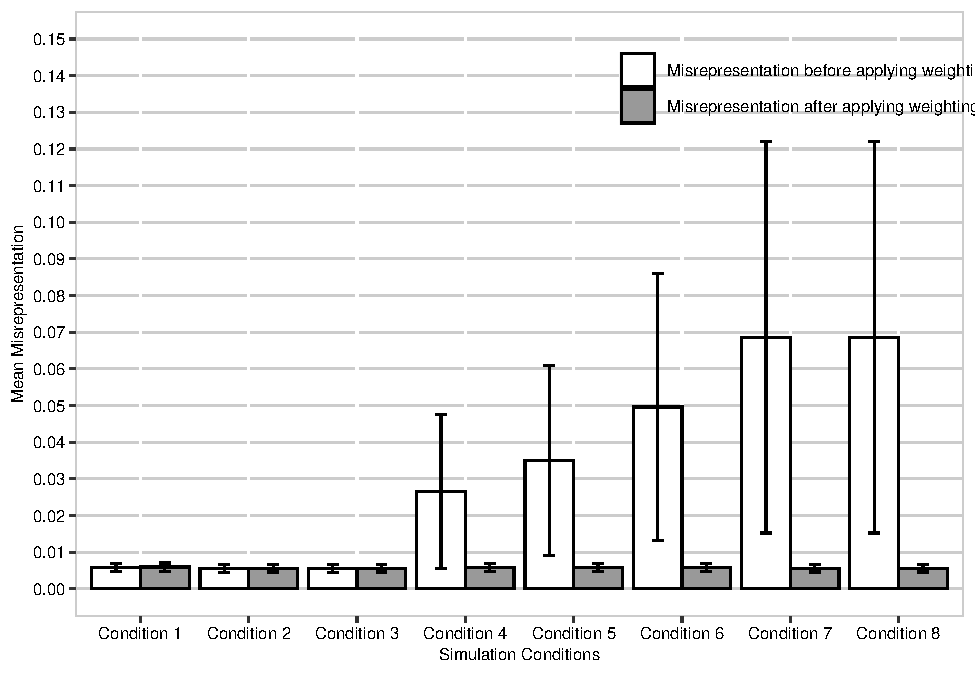
\includegraphics{Simulation-paper2-20200207_files/figure-latex/Figure4-1.pdf}
\caption{\label{fig:Figure4}Average absolute discrepancy (unweighted in white and weighted in grey) across the eight attitudinal conditions.}
\end{figure}

The plurality of our findings are presented visually, and they focus on the overall mean (e.g., the average rating across all sample members). Figure \ref{fig:Figure2} provides a broad summary of the results across the eight different attitudinal distribution conditions, presenting the average absolute discrepancy from the population mean within each broad condition. Conditions one through three demonstrate that, on average, the unweighted sample mean provides a good (unbiased) estimate of the population mean when the distributional form is held constant across constituent groups (e.g., the distributions of attitudes are of similar functional forms and locations for all constituent groups). This is regardless of form or extent of nonresponse. Additionally, weighting remediates deviations about the true mean in all five attitudinally discrepant conditions, even when considerable error exists in the unweighted estimate (e.g., the rightmost bars in Figure \ref{fig:Figure2}).

\hypertarget{the-role-of-response-rate}{%
\section{The Role of Response Rate}\label{the-role-of-response-rate}}

In terms of explaining the very little error that did emerge within the passive nonresponse conditions, this error was entirely attributable to response rate (See Figure \ref{fig:Figure3}). The nature of the exact relationship was slightly nonlinear, being fit with quadratic functions within each condition (collapsing across conditions did exhibit slight within-array differences {[}which would affect the statistically perfect relationship{]}).

\hypertarget{role-of-nonresponse-form}{%
\subsection{Role of nonresponse form}\label{role-of-nonresponse-form}}

Research question \#2 asked What role nonresponse form (passive versus active) plays in sample/population misrepresentation? \textbf{currently in paper as figures 1-3}

\begin{figure}
\centering
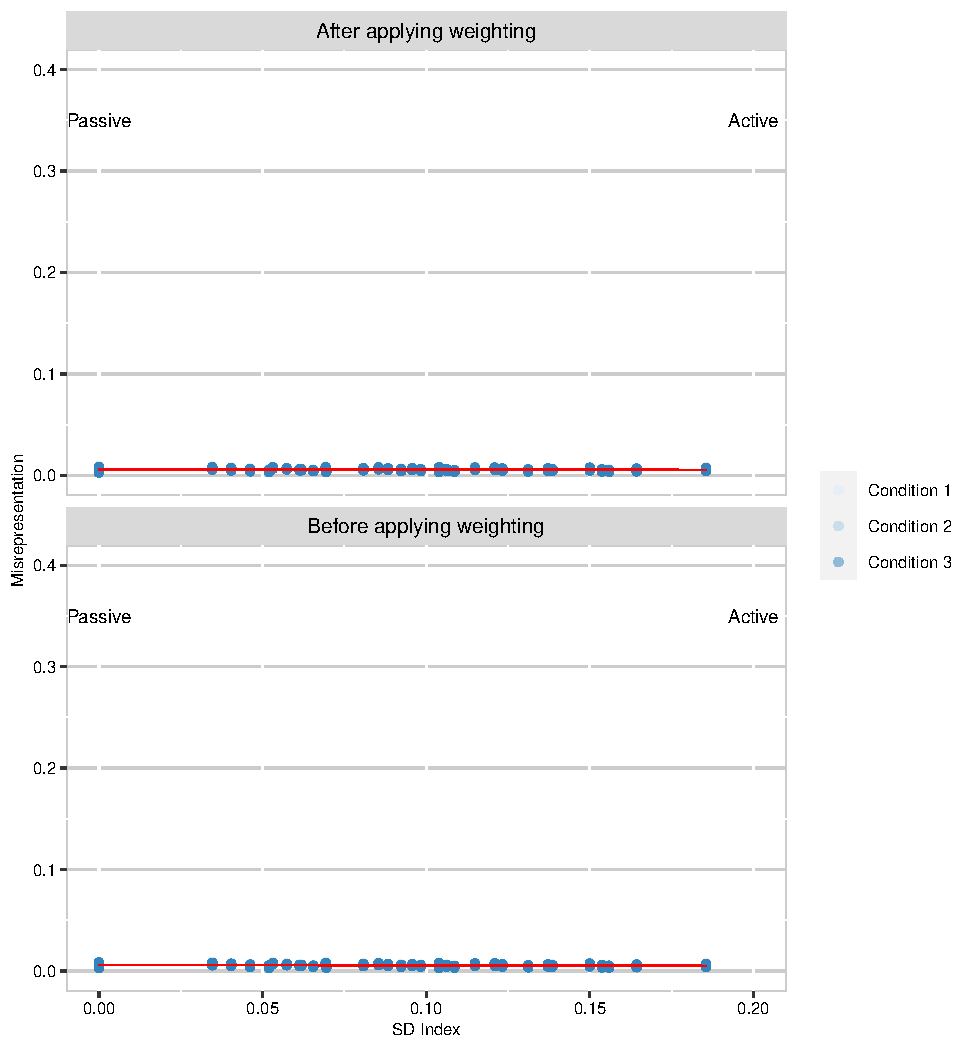
\includegraphics{Simulation-paper2-20200207_files/figure-latex/Figure5-1.pdf}
\caption{\label{fig:Figure5}Presence (or lack) of error in unweighted and weighted sample estimates across passive and active forms of nonresponse (Conditions 1 through 3).}
\end{figure}

\begin{figure}
\centering
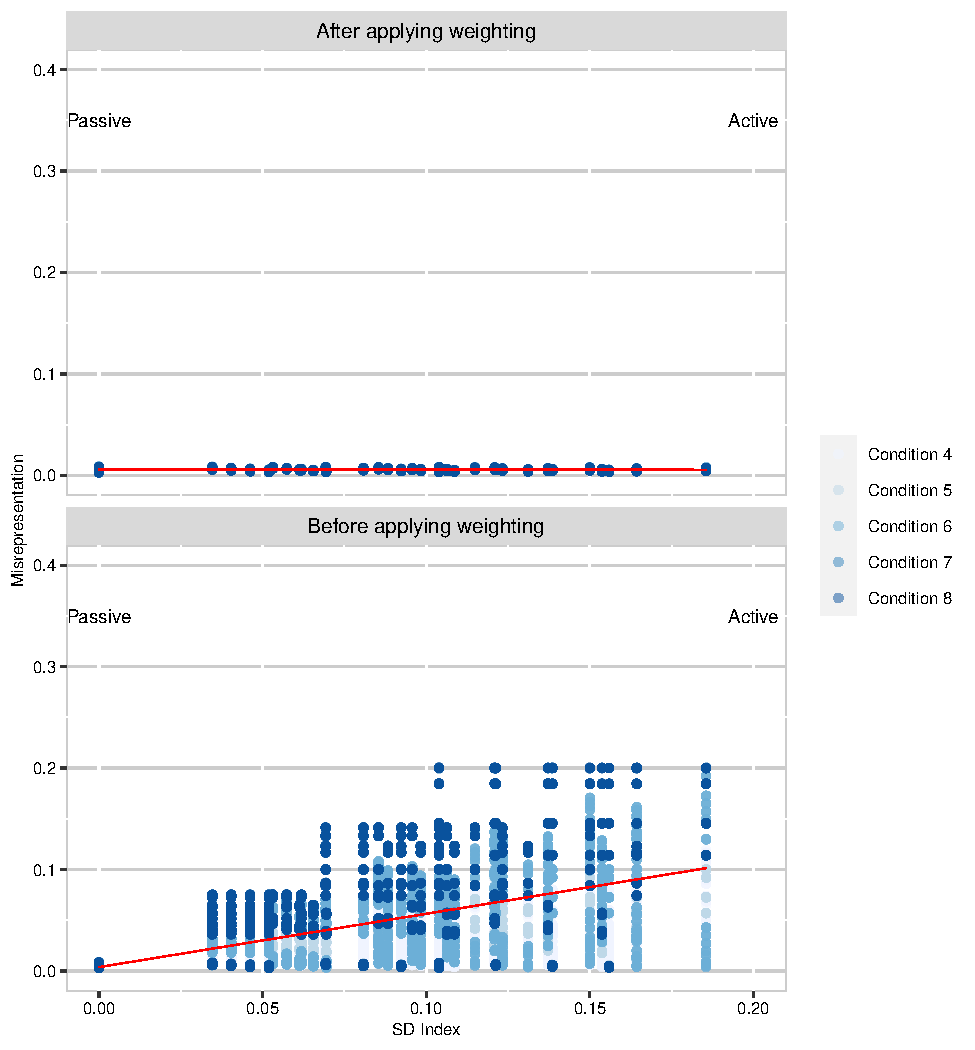
\includegraphics{Simulation-paper2-20200207_files/figure-latex/Figure6-1.pdf}
\caption{\label{fig:Figure6}Presence (or lack) of error in unweighted and weighted sample estimates across passive and active forms of nonresponse (Conditions 4 through 8).}
\end{figure}

\textbf{Need to Recall Research Questions in appropriate sections}

Figure \ref{fig:Figure4} demonstrates how the weighting algorithm operated across conditions one through three taking form of nonresponse into consideration (along the x-axis, with passive nonresponse occupying the left of the figure and active nonresponse scenarios occupying the right). There is a very slight amount of error in the unweighted sample mean with active nonresponse, as well as a systematic pattern of heteroskedasticity across the ``passive to active'' continuum (studentized Breusch-Pagan = 565.42 {[}unweighted{]}, 496.67 {[}weighted{]}, \emph{p}'s \textless{} .001). Weighting always corrects this slight amount of error. Figure 3 demonstrates a more pronounced \emph{form of} nonresponse association when underlying attitudinal distributions evidence group differences, and in these scenarios, active nonresponse is shown to have a fairly large effect on error within the sample estimate (and, again, predictable heteroskedasticity paralleling the SD index, Breusch-Pagan = 3177.2 {[}unweighted{]}; 832.91 {[}weighted{]}, \emph{p}'s \textless{} .001). Weighting again corrects the sample estimate.

It should be noted regarding the above-mentioned ``heteroskedasticity'' that there are active nonresponse scenarios in which no error is found (see, for example, the lower right-hand portion of Figure 3 where values appear all along the passive-active abscissa). These situations are ones within which the response rates ``parallel'' the distributional form. For example, in Condition Eight, the distributional forms were: Positive Skew\textsubscript{Male\_A}, Positive Skew\textsubscript{Male\_B}, Negative Skew\textsubscript{Female\_A}, Negative Skew\textsubscript{Female\_B}. In the most extreme cases of active nonresponse, response rates that fully parallel distributional patterns (e.g., 20\%\textsubscript{Male\_A}, 20\%\textsubscript{Male\_B}, 80\%\textsubscript{Female\_A}, 80\%\textsubscript{Female\_B}) result in no error in the population mean approximation (average discrepancy = .0003, \emph{SD} = .0002). Alternatively, when the response rates are inverted, (e.g., 20\%\textsubscript{Male\_A}, 80\%\textsubscript{Male\_B}, 20\%\textsubscript{Female\_A}, 80\%\textsubscript{Female\_B}), there is substantial error in approximation (average discrepancy = .51, SD = .14). \textbf{this is an old number - why are our new numbers so low? (see, for example, the y-axis on Figure 1) - YANG? (11/17/18)} Again, it is not merely response rate or form that is associated with biased sample estimates, but rather the nature of response rate relative to existing attitudinal differences.

To further elaborate this point, consider, for example, Condition 4. Here, three groups are characterized by similar distributions of attitudes (normally distributed) and one, Females from Department B, is characterized by negatively skewed attitudes. The greatest unweighted error here arises from sampling scenarios in which there are many Department B females (e.g., in our specifications, 6,400) and fewer males and Department A females\footnote{Because of the ``marginal'' versus ``cell'' specifications of population constituencies, our most extreme example here is necessarily 400 Department A males, 1,600 Department B males, and 1,600 Department A females. This was a decision based on keeping the population N's at 10,000 and certainly more extreme population constituency combinations could be examined in future like-minded explorations.}, but the Department B females exhibit a much lower response rate (e.g., 20\%) than do other groups, who respond at a high rate (e.g., 80\%). That is, it is not merely response rate, but response rate within these identifiable groups, and whether or not those response rate differences parallel underlying attitudinal differences.

Although the \emph{patterns} of unweighted sample mean discrepancies differed across conditions, all eight conditions exhibited similar omnibus effect (weighting ameliorating error wherever it arose {[}in the unweighted statistic{]}).

To partially address the second limitation, discrepancy between population constituency and sampling proportions was additionally estimated via Cattell's profile similarity index {[}\emph{r\textsubscript{p}}; Cattell (1949); Cattell et al. (1966){]}. \emph{r\textsubscript{p}} is sensitive to discrepancies in profile shape (pattern across profile components), elevation (average component score), and scatter (sum of individual components' deviation from the elevation estimate. Figure 3 demonstrates the pattern of unweighted sample mean deviation (from the population parameter) when this index is taken into consideration. \emph{edits}\ldots.again demonstrate these relationships across the attitudinal form conditions, being grouped by underlying distributions thought to be susceptible to bias (Conditions 3 through 8) as well as those thought to be relatively immune to bias (Conditions 1 through 3; aka those sampling situations in which weighting is unnecessary).

\hypertarget{summary}{%
\section{Summary}\label{summary}}

Collectively the results highlight three aspects of weighting: 1) our simulations are comprehensive, iterating through all possible combinations of response rates - those paralleling population distributions, those inversely mirroring population distributions, and those ``orthogonal to'' population distributions, 2) the ``SD'' operationalization of passive to active forms of nonresponse is a bit crude and insensitive to specific combinations of response rates expected to manifest or not manifest in bias, and 3) substantial bias may be present in the unweighted estimate even with only small proportions of active non-response (e.g., only one or two groups exhibiting slightly different response rates, with the resulting discrepancy {[}population versus sample mean{]} being quite large).

Mean square error is our second index for sample quality. It is a well-known mathematical theorem that the application of weights increases (random) errors of precision, which was also empirically true in the current study. For each condition in our simulations, we calculated the standard deviations of 40.96 million unweighted and 40.96 million weighted samples means (4,096 possible population-sample combinations by 10,000 iterations), which yielded eight empirically-estimated standard errors of unweighted and weighted sample means. Figure XXX \textbf{\textless- need to readd this} visually presents these standard errors in eight pairs of bars, demonstrating that the standard error of weighted sample means (red bar) tended to be 16\% to 18\% larger than that of unweighted sample means (grey bar) regardless of condition. These errors highlight the caveat that weighting should only be applied in the active nonresponse case (e.g., although the aggregate effect of weighting with passive nonresponse is error-minimizing, any one sampling condition is \emph{more likely} to result in greater deviation from the population parameter when weighting is applied the passive nonresponse data).

In summary, as an aggregate across sampling events, weighting always corrects sample bias, when it is present in the unweighted estimate. However, the standard errors suggest that for any \emph{one} sampling event in the absence of bias, the likelihood that the sample mean approximates the \emph{mean} of sample means is (slightly) greater for the unweighted estimate. When bias is present, however, (in the unweighted estimate) there is obviously no advantage to ``being closer'' to this biased mean of means. That is, under some circumstances, the mean of unweighted sample means does not center on the population mean. The implications of this seem quite obvious: Weighting should only be applied if bias is anticipated in the sample estimate. This may seem to be a picayune recommendation, but we note here that this advocation is not heeded in public opinion polling applications, where the computation and application of weights are default procedures (CITES? - perhaps AAPOR standards or personal communication with polling agencies such as Gallop).

\textbf{Question for David - Can we look at the ``crossing point?'' (e.g., when MSE becomes excessive)}

\hypertarget{discussion}{%
\section{Discussion}\label{discussion}}

We view nonresponse as a serious problem that should be addressed via repeated attempts to survey particularly reluctant or hard-to-reach respondents particularly because nonresponse may be reasonably expected to be greatest in groups that are most unsatisfied {[}e.g., it may be typical for individuals representing these groups to have their responses diluted; see, for example, Taris and Schreurs (2007){]}. However, several researchers have noted potentially misplaced relative emphasis on survey response rates, with Cook et al. (2000), Krosnick (1999), and Visser et al. (1996) articulating the point that representativeness of the sample is more important than response rate. We also believe that the goal in organizational surveying should be representativeness not exhaustiveness. Krosnick (1999) specifically comments that, even when probability sampling is employed, response rate does not necessarily implicate either good or poor sample representativeness. One aim of this paper is to reinforce this primary `representativeness' orientation to those who may be otherwise inclined to focus on response rate as a sufficient index of quality (and propose sample weighting as a practice that can adjust for lack of representativeness).

With the above in mind, we set out to answer two fairly simple questions: What impact does the application of weights have on the quality of sample estimates, and what role does nonresponse play? Our answers are that: 1) weighting ``always'' helps, as long as you capture the proper strata (which of course we were able to do via controlled simulation), but also 2) response rate impact \emph{depends} on relationship between response rate and the underlying distribution of attitudes. conditions 1 through 3 as well as all other conditions are occasionally immune to response rate influence, depending on whether the pattern of nonresponse parallels the pattern of attitudinal distribution differences or not). Active forms of nonresponse can harm the unweighted sample estimate, but only when the pattern of active nonresponse is accompanied by differing distributions of attitudes within the active nonrespondent ``populations'' {[}this would appear to be a reasonable expectation based on the literature; e.g., Rogelberg et al. (2000); Rogelberg et al. (2003); Spitzmüller et al. (2007){]}. Although the weighted mean proved an unbiased estimate of the population mean across all simulations, in circumstances where no bias existed in the unweighted estimate, the trade-off between bias-correction and random error of precision (e.g., standard error) also needs to be acknowledged.

It should be noted that the organizational surveying categorization of passive versus active parallels the broader statistical focus on data that is missing at random or completely at random (MAR or MCAR, see for example, Heitjan \& Basu, 1996) versus data not missing at random {[}non-MCAR, see for example, {]}. Imputation is the common remediation for data MAR or MCAR whereas non-MCAR solutions may involve strategies such as latent variable estimation procedures (Muthén et al., 1987). In the context of surveying, we are similarly proposing a bifurcation of remediation methods - no remediation with passive nonresponse and post-stratification weighting with active.

Previous presentations have noted that bias is sometimes associated with nonresponse and othertimes it is not - this research has not been explicit in the specific conditions that moderate this association, however. The current paper does make this association explicit. It is not merely the form of nonresponse that determines whether or not bias occurs, but also the underlying distributions that the response probabilities are applied to. Some distributional patterns are immune to the biasing effects of active nonresponse (see, for example, Conditions 1 through 3). Some patterns of active nonresponse also result in no bias even when distributional patterns deviate substantially (see, for example, Condition 8 where a 20\%, 20\%, 80\%, 80\% response rate pattern exhibits no error). The target therefore should not be merely form of nonresponse but also underlying attitudes. Regardless, however, weighting always remediates the error when it occurs (and does not add error where it is absent).

The current findings are of course qualified by the uniqueness of our simulations, most notably our ability to fully capture the correct population parameters (e.g., because these were ``created'' by us, we were also able to identify these strata as the nonresponse contributors). Even in the extreme conditions (e.g., a small ``population'' with a correspondingly low response rate; see, for example, the lower-left hand corner of Figure 2), the weighting algorithm was able to provide a bias correction. This is undoubtedly attributable to our random sampling procedure (instead of, for example, sampling conditionally from the population distributions), but here we do note that the raking procedure is applied at the ``margins'' (e.g., variable level, not interaction level), although our introduction of a biasing element is at the cell (interaction) level.

It has been stated that active nonresponse is relatively harmless unless the actively nonrespondent group is relatively large {[}cites below{]}. The current study, however, suggests that post-data-collection remediation. There may also be some important implications here regarding sample (and population) size. Because organizational surveyors likely interface with organizations of varying sizes (perhaps some of which are small- or medium-sized), the implications of our simulations particularly in the small population conditions, were highlighted. Findings specific to these conditions were: XXX, XXX, XXX.

There is of course no need to restrict weighting protocols to demographic groups - organizational surveyors have a rich tradition of attending to drivers of nonresponse (see, for example, Rogelberg \& Stanton, 2007). Groupings of any sort can be the basis of weighting (for example, pre-survey probing might assign probabilities of nonresponse, and these probabilities can be retained post-administration as weighting guides.

It should also be pointed out that although the active nonrespondent group seems to be a great concern, it will not seriously bias the results unless the proportion of active nonrespondents is higher than 15\% (Rogelberg et al., 2003; Rogelberg \& Stanton, 2007; Werner et al., 2007).
``In this study we found that the active nonrespondent group was relatively small (approximately 15\%), but consistent in size with research conducted by .'' (Rogelberg et al., 2003, pp. 1110--1111). ``Furthermore, consistent with Roth (1994) who stated that when missingness is not random (as we found for active nonrespondents), meaningful bias will only be introduced if the group is relatively large (which was not the case in this study).'' (Rogelberg et al., 2003, p. 1112).

``If the results show that the active nonrespondent group comprises a low proportion of the population, fewer concerns for bias arise. If the proportion of active respondents is greater than 15\% of the group of individuals included in the interviews or focus groups (this has been the average rate in other studies), generalizability may be compromised.'' (Rogelberg \& Stanton, 2007, p. 201) * I believe there is an error here. The author want to say that if the proportion of active nonrespondents is greater than 15\% of the group .

``It has been suggested that it takes a response rate of 85\% to conclude that nonresponse error is not a threat (Dooely \& Lindner, 2003). We agree that researchers should provide both empirical and theoretical evidence refuting nonresponse bias whenever the response rate is less than 85\%.'' (Werner et al., 2007, p. 293).

Note here however, the seeming disconnect between the reports of 15\% active nonresponse and declining response rates (trending toward 50\%). Certainly with decreasing overall response rates, the likely reasons would appear to be more active than passive (e.g., it is difficult to entertain the idea that potential respondents are more likely to forget to respond today than they were 40 years ago).

\begin{quote}
Integration of IT/IS systems within HR functions hopefully assists the (un)likelihood that organizatinoal population frames are either deficient or contaminated, although we note that this possibility (frame misspecification) is much more plausible within organziations that do not have updated or integrated HR IT/IS systems (perhaps, ironically, \emph{smaller} organizations).
\end{quote}

\hypertarget{future-directions}{%
\subsection{Future Directions}\label{future-directions}}

A very practical implication of this study is that future organizational researchers may find more success implementing strategic sampling strategies as opposed to (or in addition to) pursuing response enhancement. That is, as a field, organizational researchers have been focused on response-enhancing strategies that minimize the presence of nonresponse. The current findings suggest that more careful adherence to random sampling from carefully constructed population frames may provide a different route to the same end-goal of sample representativeness.

Experimental methods within the psychological discipline have long been criticized for heavy reliance on samples of convenience (for instance, student samples). Very little progress has been made regarding the application of appropriate population sampling procedures in experimentation. Certain non-experimental procedures (most notably organizational surveying) hold paradoxical advantage over experimental procedures primarily in this arena of sampling - particularly in consideration of population coverage, which refers to the percent of a population that is reachable by the sampling procedure (e.g., postal, intra-office, or internet invitation) and likelihood of having access to population parameter estimates (e.g., strata constituencies). There is a rich tradition and literature of public opinion polling procedures and techniques from which to draw. These procedures, however, only hold advantage if the non-experimental methodologist acknowledges the criticality of sample representativeness. The current paper provides one corrective technique (post-stratification weighting) as an important focus for the organizational surveyor who shares this primary interest in maximizing sample representativeness.

We note the above ``advantage'' held by organizational surveyors because extensions of the current protocol include investigating how inaccurate census estimates (and/or grabbing the ``wrong'' group) affects the quality of sample estimates. That is, in our controlled simulations, we were able to know population constituencies, because they were set by us! In real-world applications, there is likely more error between the population estimate and actual population constituency. Similarly, if the association between attitude and group membership were to be controlled, there may be conditions identified whereby weighting loses its efficacy (e.g., low ``correlations'' between attitude and group membership). Future simulations should test boundary conditions for this type of error, identifying at what point inaccuracy in the population constituency estimate appreciably degrades the weighting procedure. Furthermore, it was demonstrated here that, when bias exists, weighting corrects it. Weighting also, however, results in a larger mean square error (MSE; expected spread of sample estimates around the population parameter). Feasibly then, there is a point at which the decreased bias is accompanied by an unacceptably inflated MSE. At which point does this occur? This is another fertile area for future exploration.

Most potential issues with weighting are addressed through careful consideration of the appropriate strata to take under consideration as well as ultimate level of aggregation (what group constitutes the population of interest or focus of feedback; e.g., regional, functional, or organizational?). We recommend the surveyor especially considers groups that might have issues of active forms of nonresponse and collect those demographics so weighting is an option. It is particularly in these contexts of `unsatisfied' employees being less likely to respond to surveys that pre-stratification consideration becomes critical (for instance, if there is an inclination that attitudes may differ across, for example, night versus day shift workers, it is important that shift be measured and incorporated as a stratum prior to survey administration).

For Condition 5 (for example, low/high response rates with minority/majority population constituencies). The lower-right to upper-left diagonal reflects response rates that parallel population constituencies. The patterns across these stressors were consistent, with the weighted sample means (red dots) providing unbiased estimates of the population parameter, whereas the unweighted sample means (grey dots) tended to yield unbiased estimates when the population constituencies were roughly equal (e.g., close to 50\%/50\%).

Figure 3 drills down this information further by extracting unweighted and weighted estimates in one specific marginal population parameter combination (here, 60\% males and 40\% females; 40\% in department A and 60\% in department B). In doing so, the population parameters were in control and sample parameters were set free (see dotted red rectangle in Figure 2). Therefore, Figure 3 was then arranged in a fashion that allowed further investigation into the interactive effect of marginal sample parameters (gender on the x-axis and department on the y-axis) on the effectiveness of post-stratification weighting reflected by the pattern of grey and red dots. \textbf{Huh? - find old version or delete}

\begin{quote}
PRIOR TO RQs: after chatting with Yang (10/31/19) these need to be clarified a bit - reading 11/3 they make sense but need to be read very carefully. Check with Yang on 1/26 Skype. 2/1 revisions seem ok to Kulas. Three moving parts: underlying attitudinal distributions, response rate, and form of nonresponse \textless- perhaps we should make these variables more explicit prior to the procedure/results\ldots{}
\end{quote}

\newpage

\hypertarget{references}{%
\section{References}\label{references}}

\begingroup
\setlength{\parindent}{-0.5in}
\setlength{\leftskip}{0.5in}

\hypertarget{refs}{}
\begin{CSLReferences}{1}{0}
\leavevmode\vadjust pre{\hypertarget{ref-anseel_response_2010}{}}%
Anseel, F., Lievens, F., Schollaert, E., \& Choragwicka, B. (2010). Response rates in organizational science, 1995--2008: A meta-analytic review and guidelines for survey researchers. \emph{Journal of Business and Psychology}, \emph{25}(3), 335--349.

\leavevmode\vadjust pre{\hypertarget{ref-R-papaja}{}}%
Aust, F., \& Barth, M. (2018). \emph{{papaja}: {Create} {APA} manuscripts with {R Markdown}}. \url{https://github.com/crsh/papaja}

\leavevmode\vadjust pre{\hypertarget{ref-baruch_response_1999}{}}%
Baruch, Y. (1999). Response rate in academic studies---a comparative analysis. \emph{Human Relations}, \emph{52}(4), 421--438.

\leavevmode\vadjust pre{\hypertarget{ref-baruch_survey_2008}{}}%
Baruch, Y., \& Holtom, B. C. (2008). Survey response rate levels and trends in organizational research. \emph{Human Relations}, \emph{61}(8), 1139--1160.

\leavevmode\vadjust pre{\hypertarget{ref-biemer_introduction_2003}{}}%
Biemer, P. P., \& Lyberg, L. E. (2003). \emph{Introduction to survey quality} (Vol. 335). John Wiley \& Sons.

\leavevmode\vadjust pre{\hypertarget{ref-bobko_usefulness_2007}{}}%
Bobko, P., Roth, P. L., \& Buster, M. A. (2007). The usefulness of unit weights in creating composite scores: A literature review, application to content validity, and meta-analysis. \emph{Organizational Research Methods}, \emph{10}(4), 689--709.

\leavevmode\vadjust pre{\hypertarget{ref-cattell_r_1949}{}}%
Cattell, R. B. (1949). R p and other coefficients of pattern similarity. \emph{Psychometrika}, \emph{14}(4), 279--298.

\leavevmode\vadjust pre{\hypertarget{ref-cattell_taxonometric_1966}{}}%
Cattell, R. B., Coulter, M. A., \& Tsujioka, B. (1966). The taxonometric recognition of types and functional emergents. \emph{Handbook of Multivariate Experimental Psychology}, 288--329.

\leavevmode\vadjust pre{\hypertarget{ref-cook_meta-analysis_2000}{}}%
Cook, C., Heath, F., \& Thompson, R. L. (2000). A meta-analysis of response rates in web-or internet-based surveys. \emph{Educational and Psychological Measurement}, \emph{60}(6), 821--836.

\leavevmode\vadjust pre{\hypertarget{ref-curtin_effects_2000}{}}%
Curtin, R., Presser, S., \& Singer, E. (2000). The effects of response rate changes on the index of consumer sentiment. \emph{Public Opinion Quarterly}, \emph{64}(4), 413--428.

\leavevmode\vadjust pre{\hypertarget{ref-cycyota_enhancing_2002}{}}%
Cycyota, C. S., \& Harrison, D. A. (2002). Enhancing survey response rates at the executive level: Are employee-or consumer-level techniques effective? \emph{Journal of Management}, \emph{28}(2), 151--176.

\leavevmode\vadjust pre{\hypertarget{ref-cycyota_what_2006}{}}%
Cycyota, C. S., \& Harrison, D. A. (2006). What (not) to expect when surveying executives: A meta-analysis of top manager response rates and techniques over time. \emph{Organizational Research Methods}, \emph{9}(2), 133--160.

\leavevmode\vadjust pre{\hypertarget{ref-deming_least_1940}{}}%
Deming, W. E., \& Stephan, F. F. (1940). On a least squares adjustment of a sampled frequency table when the expected marginal totals are known. \emph{The Annals of Mathematical Statistics}, \emph{11}(4), 427--444.

\leavevmode\vadjust pre{\hypertarget{ref-fan_factors_2010}{}}%
Fan, W., \& Yan, Z. (2010). Factors affecting response rates of the web survey: A systematic review. \emph{Computers in Human Behavior}.

\leavevmode\vadjust pre{\hypertarget{ref-frohlich_techniques_2002}{}}%
Frohlich, M. T. (2002). Techniques for improving response rates in {OM} survey research. \emph{Journal of Operations Management}, \emph{20}(1), 53--62.

\leavevmode\vadjust pre{\hypertarget{ref-fulton_organizations_2016}{}}%
Fulton, B. R. (2016). Organizations and survey research: Implementing response enhancing strategies and conducting nonresponse analyses. \emph{Sociological Methods \& Research}, 0049124115626169.

\leavevmode\vadjust pre{\hypertarget{ref-heitjan_distinguishing_1996}{}}%
Heitjan, D. F., \& Basu, S. (1996). Distinguishing {``missing at random''} and {``missing completely at random.''} \emph{The American Statistician}, \emph{50}(3), 207--213.

\leavevmode\vadjust pre{\hypertarget{ref-keeter_gauging_2006}{}}%
Keeter, S., Kennedy, C., Dimock, M., Best, J., \& Craighill, P. (2006). Gauging the impact of growing nonresponse on estimates from a national {RDD} telephone survey. \emph{International Journal of Public Opinion Quarterly}, \emph{70}(5), 759--779.

\leavevmode\vadjust pre{\hypertarget{ref-kessler_national_2009}{}}%
Kessler, R. C., Avenevoli, S., Costello, E. J., Green, J. G., Gruber, M. J., Heeringa, S., Merikangas, K. R., Pennell, B.-E., Sampson, N. A., \& Zaslavsky, A. M. (2009). National comorbidity survey replication adolescent supplement ({NCS}-a): {II}. Overview and design. \emph{Journal of the American Academy of Child \& Adolescent Psychiatry}, \emph{48}(4), 380--385.

\leavevmode\vadjust pre{\hypertarget{ref-krosnick_survey_1999}{}}%
Krosnick, J. A. (1999). Survey research. \emph{Annual Review of Psychology}, \emph{50}(1), 537--567.

\leavevmode\vadjust pre{\hypertarget{ref-kulas_nonresponse_2017}{}}%
Kulas, J. T., Robinson, D. H., Kellar, D. Z., \& Smith, J. A. (2017). Nonresponse in organizational surveying: Attitudinal distribution form and conditional response probabilities' impact on patterns of bias. \emph{Public Opinion Quarterly}, \emph{81}(2), 401--421.

\leavevmode\vadjust pre{\hypertarget{ref-kulas_post-stratification_2016}{}}%
Kulas, J. T., Robinson, D. H., Smith, J. A., \& Kellar, D. Z. (2016). Post-stratification weighting in organizational surveys: A cross-disciplinary tutorial. \emph{Human Resource Management}.

\leavevmode\vadjust pre{\hypertarget{ref-landers_inconvenient_2015}{}}%
Landers, R. N., \& Behrend, T. S. (2015). An inconvenient truth: Arbitrary distinctions between organizational, mechanical turk, and other convenience samples. \emph{Industrial and Organizational Psychology}, \emph{8}(2), 142--164.

\leavevmode\vadjust pre{\hypertarget{ref-luong_how_1998}{}}%
Luong, A., \& Rogelberg, S. G. (1998). How to increase your survey response rate. \emph{The Industrial-Organizational Psychologist}, \emph{36}(1), 61--65.

\leavevmode\vadjust pre{\hypertarget{ref-mellahi_response_2016}{}}%
Mellahi, K., \& Harris, L. C. (2016). Response rates in business and management research: An overview of current practice and suggestions for future direction. \emph{British Journal of Management}, \emph{27}(2), 426--437.

\leavevmode\vadjust pre{\hypertarget{ref-muthen_structural_1987}{}}%
Muthén, B., Kaplan, D., \& Hollis, M. (1987). On structural equation modeling with data that are not missing completely at random. \emph{Psychometrika}, \emph{52}(3), 431--462.

\leavevmode\vadjust pre{\hypertarget{ref-R-anesrake}{}}%
Pasek, J. (2018). \emph{Anesrake: ANES raking implementation}. \url{https://CRAN.R-project.org/package=anesrake}

\leavevmode\vadjust pre{\hypertarget{ref-pedersen_improving_2016}{}}%
Pedersen, M. J., \& Nielsen, C. V. ek. (2016). Improving survey response rates in online panels: Effects of low-cost incentives and cost-free text appeal interventions. \emph{Social Science Computer Review}, \emph{34}(2), 229--243.

\leavevmode\vadjust pre{\hypertarget{ref-quine_feeling_2008}{}}%
Quine, S., \& Morrell, S. (2008). Feeling safe in one's neighbourhood: Variation by location among older australians. \emph{The Australian Journal of Rural Health}, \emph{16}, 115--116.

\leavevmode\vadjust pre{\hypertarget{ref-rivers_inference_2009}{}}%
Rivers, D., \& Bailey, D. (2009). Inference from matched samples in the 2008 {US} national elections. \emph{Proceedings of the Joint Statistical Meetings}, \emph{1}, 627--639.

\leavevmode\vadjust pre{\hypertarget{ref-rogelberg_profiling_2003}{}}%
Rogelberg, S. G., Conway, J. M., Sederburg, M. E., Spitzmüller, C., Aziz, S., \& Knight, W. E. (2003). Profiling active and passive nonrespondents to an organizational survey. \emph{Journal of Applied Psychology}, \emph{88}(6), 1104.

\leavevmode\vadjust pre{\hypertarget{ref-rogelberg_employee_2000}{}}%
Rogelberg, S. G., Luong, A., Sederburg, M. E., \& Cristol, D. S. (2000). Employee attitude surveys: Examining the attitudes of noncompliant employees. \emph{Journal of Applied Psychology}, \emph{85}(2), 284.

\leavevmode\vadjust pre{\hypertarget{ref-rogelberg_introduction_2007}{}}%
Rogelberg, S. G., \& Stanton, J. M. (2007). \emph{Introduction: Understanding and dealing with organizational survey nonresponse}. Sage Publications Sage {CA}: Los Angeles, {CA}.

\leavevmode\vadjust pre{\hypertarget{ref-spitzmuller_survey_2007}{}}%
Spitzmüller, C., Glenn, D. M., Sutton, M. M., Barr, C. D., \& Rogelberg, S. G. (2007). Survey nonrespondents as bad soldiers: Examining the relationship between organizational citizenship and survey response behavior. \emph{International Journal of Selection and Assessment}, \emph{15}(4), 449--459.

\leavevmode\vadjust pre{\hypertarget{ref-taris_how_2007}{}}%
Taris, T. W., \& Schreurs, P. J. (2007). How may nonresponse affect findings in organizational surveys? The tendency-to-the-positive effect. \emph{International Journal of Stress Management}, \emph{14}(3), 249.

\leavevmode\vadjust pre{\hypertarget{ref-tett_2011_2014}{}}%
Tett, R., Brown, C., \& Walser, B. (2014). The 2011 {SIOP} graduate program benchmarking survey part 7: Theses, dissertations, and performance expectations. \emph{The Industrial-Organizational Psychologist}, \emph{51}(4), 62--73.

\leavevmode\vadjust pre{\hypertarget{ref-visser_mail_1996}{}}%
Visser, P. S., Krosnick, J. A., Marquette, J., \& Curtin, M. (1996). Mail surveys for election forecasting? An evaluation of the columbus dispatch poll. \emph{Public Opinion Quarterly}, \emph{60}(2), 181--227.

\leavevmode\vadjust pre{\hypertarget{ref-wainer_estimating_1976}{}}%
Wainer, H. (1976). Estimating coefficients in linear models: It don't make no nevermind. \emph{Psychological Bulletin}, \emph{83}(2), 213.

\leavevmode\vadjust pre{\hypertarget{ref-werner_reporting_2007}{}}%
Werner, S., Praxedes, M., \& Kim, H.-G. (2007). The reporting of nonresponse analyses in survey research. \emph{Organizational Research Methods}, \emph{10}(2), 287--295.

\end{CSLReferences}

\endgroup


\end{document}
